\pgfmathsetseed{123456789}%
\tikzset{expressed/.style={-stealth,shorten <=4pt,shorten >=6pt,ultra thick}}%
\tikzset{potential/.style={-stealth,shorten <=4pt,shorten >=6pt,very thick,dotted}}%
\usetikzlibrary{calc}

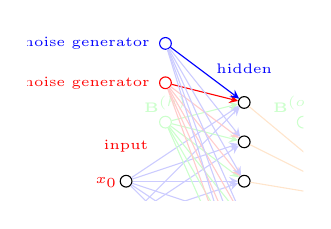
\begin{tikzpicture}
\clip (-1.25,2) rectangle + (3.5,2.2);
	\foreach \i in {0,...,1} \node[draw,circle,inner sep=1.5pt] (input\i) at (0,\the\numexpr0.5*\i+1.0+0.75) {};
	\foreach \i in {0,...,5} \node[draw,circle,inner sep=1.5pt] (hidden\i) at (1.5,\the\numexpr0.5*\i+0.75) {};
    \foreach \i in {0,...,0} \node[draw,circle,inner sep=1.5pt] (output\i) at (3.0,\the\numexpr0.5*\i+1.25+.75) {};

    % connectors input -> hidden
	\foreach \i in {0,...,1}
		\foreach \j in {0,...,5} \draw[-stealth,blue!20!white] (input\i) -- (hidden\j);

    % connectors hidden -> output
	\foreach \i in {0,...,5}
		\foreach \j in {0,...,0} \draw[-stealth,orange!20!white] (hidden\i) -- (output\j);

    % labels
	\draw (input1) ++ (0.0,0.25) node[red,above] {\tiny input};
	\draw (input0) ++ (-0.25,-0.20) node[red!100!white,above] {\tiny $x_1$};
	\draw (input1) ++ (-0.25,-0.20) node[red!100!white,above] {\tiny $x_0$};
	\draw (hidden5) ++ (0.0,0.25) node[blue,above] {\tiny hidden};
	\draw (output0) ++ (0.0,0.25) node[orange,above] {\tiny output};
	\draw (output0) ++ (0.25,-0.20) node[orange,above] {\tiny y};		
    
    % bias nodes
    \node[color=green!20!white,draw,circle,inner sep=1.5pt] (bias1) at (0.5,5*0.5+0.5) {};
	\draw (bias1) ++ (0.0,0.0) node[green!20!white,above] {\tiny $\textbf{B}^{\text{(h)}}$};
	
    \node[color=green!20!white,draw,circle,inner sep=1.5pt] (bias2) at (2.25,5*0.5+0.5) {};
	\draw (bias2) ++ (0.0,0.0) node[green!20!white,above] {\tiny $\textbf{B}^{\text{(out)}}$};

    % bias connectors
	\foreach \i in {0,...,5} \draw[-stealth,green!20!white] (bias1) -- (hidden\i);
	\draw[-stealth,green!20!white] (bias2) -- (output0);
    
	% weight labels
	\draw (input0) ++ (0.5,-1.0) node[blue!20!white,above] {\tiny $\textbf{W}^{\text{(h)}}$};
	\draw (hidden0) ++ (1.1,0) node[orange!20!white,above] {\tiny $\textbf{W}^{\text{(out)}}$};

    % noise generators
    \node[color=red!100!white,draw,circle,inner sep=1.5pt] (noise1) at (0.5,5*0.5+0.5+0.5) {};
	\draw (noise1) ++ (-1.,-0.2) node[red!100!white,above] {\tiny noise generator};
    \node[color=blue!100!white,draw,circle,inner sep=1.5pt] (noise2) at (0.5,5*0.5+0.5+1.0) {};
	\draw (noise2) ++ (-1.0,-0.2) node[blue!100!white,above] {\tiny noise generator};
    
    % noise connectors
    \draw[-stealth,red!100!white] (noise1) -- (hidden5);
    \draw[-stealth,blue!100!white] (noise2) -- (hidden5);
	\foreach \i in {0,...,4} \draw[-stealth,red!20!white] (noise1) -- (hidden\i);
	\foreach \i in {0,...,4} \draw[-stealth,blue!20!white] (noise2) -- (hidden\i);
	
	 \node[draw,color=white] (dummy) at (0,0.5) {};
\end{tikzpicture}